\chapter{Figuras anat\'omicas de referencia}

Las figuras de este anexo son esquem\'aticas y tienen finalidad exclusivamente explicativa. No representan un estudio cl\'inico real ni deben utilizarse para interpretaci\'on diagn\'ostica. Su objetivo es facilitar la comprensi\'on general de las estructuras anat\'omicas consideradas por el prototipo y del flujo conceptual de segmentaci\'on utilizado en el proyecto.

\section{Esquema simplificado de columna lumbar sagital}

\begin{figure}[H]
\centering
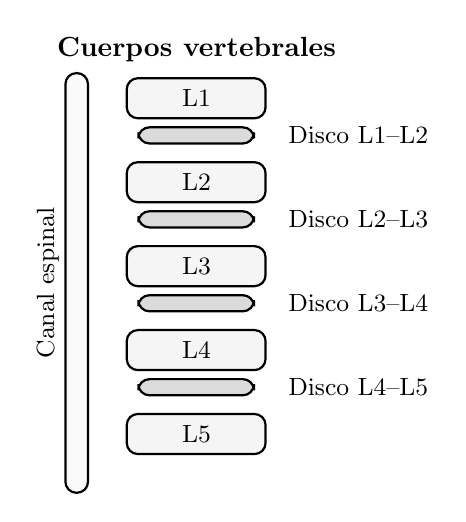
\begin{tikzpicture}[
    scale=0.82,
    font=\small,
    vertebra/.style={draw, thick, rounded corners, fill=gray!8},
    disc/.style={draw, thick, rounded corners, fill=gray!28},
    canal/.style={draw, thick, rounded corners, fill=gray!5}
]
    % Canal espinal
    \draw[canal] (-0.95,0.45) rectangle (-0.60,6.95);
    \node[rotate=90] at (-1.22,3.7) {Canal espinal};

    % Vertebras
    \foreach \y/\label in {6.25/L1,4.95/L2,3.65/L3,2.35/L4,1.05/L5} {
        \draw[vertebra] (0,\y) rectangle (2.15,\y+0.62);
        \node at (1.08,\y+0.31) {\label};
    }

    % Discos
    \foreach \y/\label in {5.86/L1--L2,4.56/L2--L3,3.26/L3--L4,1.96/L4--L5} {
        \draw[disc] (0.18,\y) rectangle (1.97,\y+0.25);
        \node[anchor=west] at (2.35,\y+0.13) {Disco \label};
    }

    \node[font=\bfseries] at (1.08,7.32) {Cuerpos vertebrales};
\end{tikzpicture}
\caption{Esquema simplificado de v\'ertebras lumbares, discos intervertebrales y canal espinal en vista sagital. Elaboraci\'on propia.}
\label{fig:esquema-lumbar-sagital}
\end{figure}

\section{Esquema conceptual de segmentaci\'on}

\begin{figure}[H]
\centering
\resizebox{\textwidth}{!}{%
\begin{tikzpicture}[
    font=\small,
    box/.style={draw, rounded corners, minimum width=3.4cm, minimum height=3.0cm, align=center},
    maskbox/.style={draw, rounded corners, minimum width=3.8cm, minimum height=3.0cm, align=center},
    modelbox/.style={draw, rounded corners, minimum width=2.7cm, minimum height=1.2cm, align=center, fill=gray!10},
    arrow/.style={-{Stealth}, thick},
    vertebra/.style={draw, rounded corners, fill=gray!10},
    disc/.style={draw, rounded corners, fill=gray!35},
    canal/.style={draw, fill=gray!5}
]

% Bloque 1: imagen RM
\node[box] (rm) at (0,0) {};
\node[above=0.15cm of rm] {\textbf{Imagen de RM lumbar}};

% Contenido RM
\draw[canal] (-1.25,-1.15) rectangle (-1.10,1.15);
\foreach \y in {0.8,0.0,-0.8} {
    \draw[vertebra] (-0.65,\y-0.18) rectangle (0.55,\y+0.18);
}
\foreach \y in {0.4,-0.4} {
    \draw[disc] (-0.55,\y-0.06) rectangle (0.45,\y+0.06);
}

% Bloque 2: modelo
\node[modelbox] (model) at (4.9,0) {\textbf{Modelo IA}\\Segmentaci\'on};

% Bloque 3: mascaras
\node[maskbox] (masks) at (9.8,0) {};
\node[above=0.15cm of masks] {\textbf{M\'ascaras generadas}};

% Mini mascaras / leyenda
\draw[vertebra] (8.25,0.65) rectangle (8.85,0.95);
\node[anchor=west] at (9.15,0.80) {V\'ertebras};

\draw[disc] (8.25,0.10) rectangle (8.85,0.28);
\node[anchor=west] at (9.15,0.19) {Discos};

\draw[canal] (8.45,-0.95) rectangle (8.65,-0.35);
\node[anchor=west] at (9.15,-0.65) {Canal espinal};

% Flechas
\draw[arrow] (rm.east) -- (model.west);
\draw[arrow] (model.east) -- (masks.west);

\end{tikzpicture}
}
\caption{Esquema conceptual del pasaje desde una RM lumbar hacia m\'ascaras de segmentaci\'on. Elaboraci\'on propia.}
\label{fig:esquema-segmentacion}
\end{figure}
